
\documentclass[titlepage = firstcover]{scrartcl}
\usepackage[aux]{rerunfilecheck}
\usepackage{fontspec}
\usepackage[main=ngerman, english, french]{babel}

% mehr Pakete hier
\usepackage{expl3}
\usepackage{xparse}
\usepackage{graphicx}

%Mathematik------------------------------------------------------
\usepackage{amsmath}   % unverzichtbare Mathe-Befehle
\usepackage{amssymb}   % viele Mathe-Symbole
\usepackage{mathtools} % Erweiterungen für amsmath
\usepackage[
  math-style=ISO,    % \
  bold-style=ISO,    % |
  sans-style=italic, % | ISO-Standard folgen
  nabla=upright,     % |
  partial=upright,   % /
]{unicode-math}% "Does exactly what it says on the tin."



% Laden von OTF-Mathefonts
% Ermöglich Unicode Eingabe von Zeichen: α statt \alpha

\setmathfont{Latin Modern Math}
%\setmathfont{Tex Gyre Pagella Math} % alternativ zu Latin Modern Math
\setmathfont{XITS Math}[range={scr, bfscr}]
\setmathfont{XITS Math}[range={cal, bfcal}, StylisticSet=1]

\AtBeginDocument{ % wird bei \begin{document}
  % werden sonst wieder von unicode-math überschrieben
  \RenewDocumentCommand \Re {} {\operatorname{Re}}
  \RenewDocumentCommand \Im {} {\operatorname{Im}}
}
\usepackage{mleftright}
\setlength{\delimitershortfall}{-1sp}

%Sprache----------------------------------------------------------
\usepackage{microtype}
\usepackage{xfrac}
\usepackage[autostyle]{csquotes}    % babel
\usepackage[unicode, pdfusetitle]{hyperref}
\usepackage{bookmark}
\usepackage[shortcuts]{extdash}
%Einstellungen hier, z.B. Fonts
\usepackage{booktabs} % Tabellen

%Defininierte funktionen
\DeclareMathOperator{\f}{xyz}

\ExplSyntaxOn % bequeme Syntax für Definition von Befehlen

\NewDocumentCommand \I {} {         %Befehl \I definieren,keine Argumente
  \symup{i}                         %Ergebnis von \I
} 
\NewDocumentCommand \dif {m} % m = mandatory (Pflichtargument für \dif)
{
  \mathinner{\symup{d} #1}
}

\ExplSyntaxOff % Syntax wieder ausschalten. Wichtig!

\setlength{\parindent}{0pt} % Einrückung bei neuem Absatz ausschalten
%\addtolength{\parskip}{\baselineskip} % Eine Leerzeile Abstand vor Absatz

%\RedeclareSectionCommand[ % Abstand vor und nach section
  %beforeskip=-1\baselineskip,
  %afterskip=.25\baselineskip]{section}


\title{Das Hooksche Gesetz}
\author{David Gutnikov \and Lasse Sternemann}
\date{22.10.19}

\begin{document}
    \maketitle


    \section{Versuchsbeschreibung}
        In diesem Versuch geht es darum, den Zusammenhang zwischen der auf die Feder wirkenden Kraft und der Federauslenkung zu bestimmen.
        Die Feder hängt an einem Kraftmesser, der die an der Feder anliegende Kraft F misst. Zudem ist an der Feder ein Seil befestigt, 
        welches über eine Umlenkrolle entlang eines Maßstabs gezogen werden kann. So lässt sich die Auslenkung der Feder in Abhängigkeit zu
        der angreifenden Kraft ablesen.

    \section{Versuchsdurchführung}
        Zuerst wird das Seil so gestrafft, dass sich die Feder trotzdem noch in ihrer Ruhelage befindet. Nun wird graduell die Auslenkung der 
        Feder in Intervallen von je 5 Zentimetern erhöht. Dabei wird nach jeder Erhöhung die auf die Feder wirkende Kraft notiert.

        
    \section{Bestimmung der Federkonstante}

      \subsection{Mittelwert}
        Nun wollen wir die Federkonstante bestimmen. Dazu stellen wir das Hooksche Gesetz nach D um.

        \begin{equation}
            F = D \cdot \Delta x  \qquad \Leftrightarrow  \qquad D = \frac{F}{\Delta x}
        \end{equation} 

      

        Mit der obrigen Formel berechnen wir mit unseren Messwerten die einzelnen Federkonstanten. 

        \begin{table}[h]
          \centering
          \caption{Messdaten}
          \label{tab:Tabelle_1}
          
          \begin{tabular}{c c c}
              \toprule
              {$\Delta x$ \ [cm]} & {$F$ \ [N]} & {$D$ \ [$\frac{N}{cm}$]}\\
              \midrule
              5 & 0,15 & 0.03000\\
              10 & 0,29 & 0.02900\\
              15 & 0,44 & 0.02933\\
              20 & 0,59 & 0.02950\\
              25 & 0,74 & 0.02960\\
              30 & 0,89 & 0.02967\\
              35 & 1,04 & 0.02971\\
              40 & 1,19 & 0.02975\\
              45 & 1.34, & 0.02978\\
              50 & 1,49 & 0.02980\\
              \bottomrule
          \end{tabular}    
      \end{table}

      \newpage
      Zudem berechnen wir mit der folgenden Formel den Mittelwert für die Federkonstante 
        \begin{equation}
          \bar{D} = \frac{1}{n} \cdot \sum_{i=1}^{n} D_{i}
        \end{equation}  
      und kommen auf $\bar{D}$ = 0,0296 . 

        
      \subsection{Lineare Regression}
        Nun tragen wir unsere Messwerte in einem Diagramm auf. Über diese Werte legen wir
        eine Ausgleichsgerade, die aus den gemessenen Auslenkungen und dem Mittelwert der Federkonstanten hervorgeht.
        
        \begin{center}
          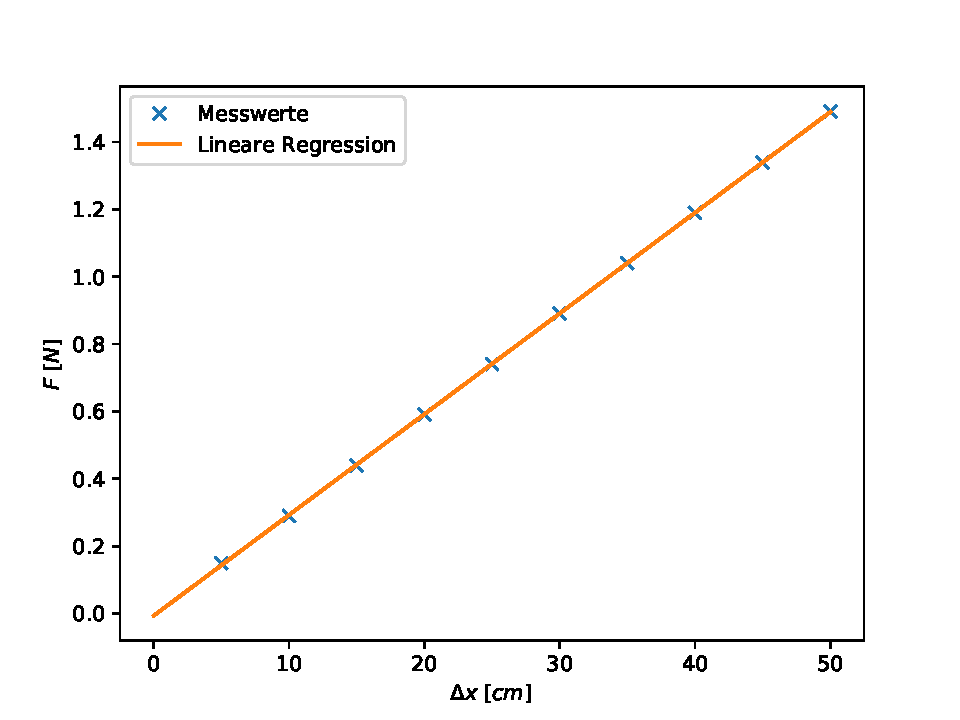
\includegraphics[width=0.6\linewidth]{Hookgraph.pdf}
        \end{center}

        Die Steigung der Ausgleichsgerade soll das $D$ sein und liegt bei 0,0299. Der y-Achsenabschnitt ist -0,0060.

        \end{document}